\documentclass{article}
\usepackage{graphicx}

\title{Labwork 5: Gaussian Blur Convolution}
\author{Nguyen Nhu Duy}
\date{}

\begin{document}

\maketitle

\section{Implementation}

A 7$\times$7 Gaussian blur filter was implemented using a 2D CUDA kernel.
Each thread processes one image pixel and applies the Gaussian filter to its local neighborhood.

Two GPU versions were tested:
\begin{itemize}
    \item Without shared memory.
    \item With shared memory, where the Gaussian filter is copied to shared memory.
\end{itemize}

A CPU implementation was also tested for comparison.

\section{Experiment}

The following block sizes were tested: (8,8),\ (16,16),\ (32,16),\ (16,32),\ (32,32)

The execution time was measured using \texttt{time.time()}.
A warm-up run was performed before timing, and each result is the average of five runs.

The CPU execution time was approximately: 2400.61 s.


Without shared memory, the fastest result was obtained with block size
$(16,16)$ at approximately $0.000165$ s.

With shared memory, the fastest result was obtained with block size
$(32,16)$ at approximately $0.05823$ s.

\begin{center}
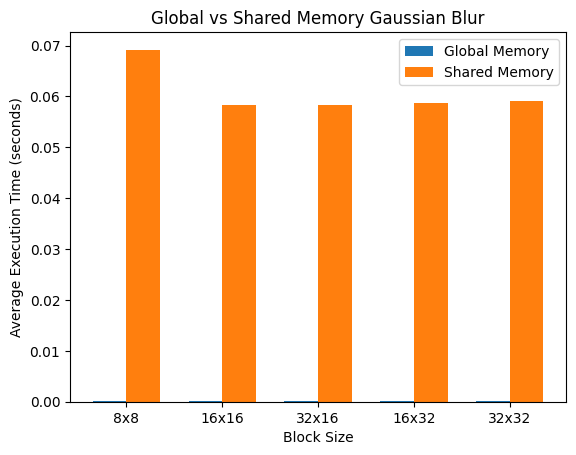
\includegraphics[width=0.8\textwidth]{gaussian_blur_compare.png}
\end{center}

\section{Discussion}

The GPU implementation was much faster than the CPU implementation.
However, in this experiment, the shared-memory version was slower than
the version without shared memory.

The additional time is caused by the overhead of copying the filter into
shared memory and synchronizing threads. Therefore, shared memory does not
always improve performance when the synchronization and memory-management
overhead is larger than the benefit.

\end{document}